
%% bare_conf.tex
%% V1.3
%% 2007/01/11
%% by Michael Shell
%% See:
%% http://www.michaelshell.org/
%% for current contact information.
%%
%% This is a skeleton file demonstrating the use of IEEEtran.cls
%% (requires IEEEtran.cls version 1.7 or later) with an IEEE conference paper.
%%
%% Support sites:
%% http://www.michaelshell.org/tex/ieeetran/
%% http://www.ctan.org/tex-archive/macros/latex/contrib/IEEEtran/
%% and
%% http://www.ieee.org/

%%*************************************************************************
%% Legal Notice:
%% This code is offered as-is without any warranty either expressed or
%% implied; without even the implied warranty of MERCHANTABILITY or
%% FITNESS FOR A PARTICULAR PURPOSE!
%% User assumes all risk.
%% In no event shall IEEE or any contributor to this code be liable for
%% any damages or losses, including, but not limited to, incidental,
%% consequential, or any other damages, resulting from the use or misuse
%% of any information contained here.
%%
%% All comments are the opinions of their respective authors and are not
%% necessarily endorsed by the IEEE.
%%
%% This work is distributed under the LaTeX Project Public License (LPPL)
%% ( http://www.latex-project.org/ ) version 1.3, and may be freely used,
%% distributed and modified. A copy of the LPPL, version 1.3, is included
%% in the base LaTeX documentation of all distributions of LaTeX released
%% 2003/12/01 or later.
%% Retain all contribution notices and credits.
%% ** Modified files should be clearly indicated as such, including  **
%% ** renaming them and changing author support contact information. **
%%
%% File list of work: IEEEtran.cls, IEEEtran_HOWTO.pdf, bare_adv.tex,
%%                    bare_conf.tex, bare_jrnl.tex, bare_jrnl_compsoc.tex
%%*************************************************************************

% *** Authors should verify (and, if needed, correct) their LaTeX system  ***
% *** with the testflow diagnostic prior to trusting their LaTeX platform ***
% *** with production work. IEEE's font choices can trigger bugs that do  ***
% *** not appear when using other class files.                            ***
% The testflow support page is at:
% http://www.michaelshell.org/tex/testflow/

\documentclass[conference, 10pt]{IEEEtran}

\usepackage{graphicx}
\usepackage{color}
\usepackage{placeins}
\usepackage{float}
\usepackage{tabularx,colortbl}
\usepackage{algpseudocode}
\usepackage{algorithm}
\usepackage{qtree}
\usepackage{url}
\usepackage{pgfplots}
\usepackage[section,subsection]{extraplaceins}
\usepackage{tikz}
\usetikzlibrary{shadings}
\definecolor{eggshell}{RGB}{252,230,201}
\pgfdeclareradialshading{eggshading}{\pgfpoint{1cm}{1cm}}%
{color(0cm)=(eggshell!80);
color(0.5cm)=(brown!75!eggshell);
color(0.7cm)=(brown);
color(0.9cm)=(brown!70!black);
color(1.2cm)=(black)
}
\pgfdeclareradialshading{eggshadow}{\pgfpointorigin}%
{color(0cm)=(black);
color(2mm)=(gray!80);
color(3mm)=(gray!40);
%color(0.3cm)=(black!5!white);
color(7mm)=(white)
}

\begin{document}
%
% paper title
% can use linebreaks \\ within to get better formatting as desired
\title{Spatial Clustering Algorithms: A Selective Survey}


% author names and affiliations
% use a multiple column layout for up to three different
% affiliations
\author{\IEEEauthorblockN{Baskin, Sean \\
                          Reinsmidt, Eric \\
                          Sidella, Pallavi}
\IEEEauthorblockA{Department of Engineering and Computer Science\\
University of Tennessee at Chattanooga\\
Chattanooga, Tennessee, U.S.A.\\}}

% make the title area
\maketitle


\begin{abstract}
%\boldmath
% Please include a brief abstract here. The abstract should be limited to 50-200 words and should concisely state what was done, how it was done, principal results, and their significance.

This report presents a selective survey of spatial clustering algorithms that includes BIRCH, DBSCAN, and Fuzzy K-Means. The focus of this survey is to provide a comparison of each algorithm's asymptotic running-time and experimental results.

Our research involves determining which of the selected algorithms provides the most efficient estimated runtime and most efficient experimental runtime in a real-world implementation with regard to spatial-specific metrics including: the ability to handle dimensionality, ability to hndle irregularly shaped clusters, insensitivity to noise, and independence of the data input order.

The algorithms were evaluated using a data set from the National Oceanic and Atmospheric Administration (NOAA), which was comprised of hail storm data from 1955 - 2011. The evaluation ran each algorithm on recursive subsets of the dataset of size $[n/2]$ and recording their run time for each subset. The asymptotic running time correlates strongly with the empirical results, validating the use of asymtotic analysis.

\end{abstract}

\section{Introduction}
With the pervasiveness of localized and continuous data collection, the amount of data available has increased exponentially. Clustering is a technique used in knowledge discovery and data mining (KDD) and is also common in statistical data analysis \cite{survey}. Spatial data spans the range of nominal, ordinal, interval, and ratio levels of measurement and can be continuous or discrete \cite{spat}. Clustering techniques can be extended to spatial data for KDD. Clustering roughly falls within three broad categories: partition-based, hierachical, and locality clustering \cite{spatial}

 As the name suggests, partition based clustering partitions the data into groups of similar objects in a cluster compared to the objects in other clusters.  K-means, K-medoids and Fuzzy C means are few of the popular partition-based clustering algorithms.  Hierarchical clustering is based on the idea of building a tree of data that can merge similar groups of points together by performing a sequence of partitions. BIRCH, CHAMELEON, and CURE are some of the examples of hierarchical clustering.  Density based clustering is based on grouping of clusters as areas of higher density than the remaining data. DBSCAN, GDBSCAN and OPTICS are some of the examples of density based clustering. Out of each the three general types of spatial clustering algorithms, we have chosen one algorithm to run performance testing.

%==================================
% BIRCH ALGORITHM
%==================================
\subsection{BIRCH}

The Balanced Iterative Reducing and Clustering using Hierarchies (BIRCH) algorithm was conceived of as a way to balance the need to cluster extremely large data sets in situations where time and memory are limited \cite{birch}. To achieve the time requirement, BIRCH only scans a data set one time, which improves the rumtime efficiency. While it may be counterintuitive that it only scans a data set one time while also having a memory restricted system, BIRCH accomplishes this by building a Clustering Feature Tree (CF Tree) that can cluster data in chunks as it is scanned piecemeal \cite{birch}.

The BIRCH algorithm consists of four phases, two of which are optional:
\vspace{1 mm}
\begin{enumerate}
  \item Creation of the CF Tree scanned into memory in $O(n)$
  \item Resizing tree to remove outliers (optional)
  \item Clustering using custom hierarchichal agglomerative clustering algorithm in $O(n^2)$
  \item Additional scanning of the data for improved outlier removal (optional)
\end{enumerate}
\vspace{1 mm}

The heart of the BIRCH algorithm is the CF Tree, which is a dendrogram comprised of internal nodes and leaf nodes. The CF Tree's nodes are comprised of three pieces of data:\vspace{1 mm}
$N$, the total number of objects in the node\\*
$LS$, the linear sum of the $N$ data points\\*
For internal nodes
\begin{equation}
\overrightarrow{LS} = \sum_{i=1}^{k}\overrightarrow{LS}\:\:of\:\:N_i
\end{equation}
For leaf nodes
\begin{equation}
LS = \sum_{P_i\epsilon N}^{ }P_i
\end{equation}
$SS$, the square sum of the $N$ data points\\*
For internal nodes
\begin{equation}
SS = \sum_{i=1}^{k}SS\:\:of\:\:N_i
\end{equation}
For leaf nodes
\begin{equation}
SS = \sum_{P_i\epsilon N}^{ }\left | P_i\right |^2
\end{equation}

\begin{figure}[!hb]
    \centering
    \includegraphics[width=90mm]{cf_tree.png}
    \caption{CF Tree Example}
\end{figure}

Beyond the CF Tree, BIRCH has more important elements:\vspace{1 mm}
$B$ the branching factor, i.e how many children an internal node can have\\*
$T$ the threshold, i.e. how many CF data points are allowed in a node\\*
$L$ the leaf threshold, i.e. how many CF data points are allowed in a leaf node\\*

\begin{algorithm}
\caption{BIRCH - Phase 1}
\begin{algorithmic}[1]
  \Procedure{BirchTreeBuilder}{$i$, $node$}
    \State Input: $D$ (set with $n$ points), $root$ (root of CF Tree)
    \State Output: CF Tree
    \For{$i\gets 1, n$}
      \State{Insert value $i$ into $root$}
      \If{$i$ closest to current node}
        \State{insert $i$ into current node}
        \Else
        \State{BirchTreeBuilder($i$, $node.children$)}
      \EndIf
    \EndFor
  \EndProcedure
\end{algorithmic}
\end{algorithm}

\begin{algorithm}
\caption{BIRCH - Phase 3}
\begin{algorithmic}[1]
  \Procedure{Clustering}{}
    \State Input: $L$ (set with $n$ leaf nodes in CF Tree)
    \State Output: Clusters
    \While{$n > 1$}
      \State{$closest = \infty$}
      \State{$left = null, right = null$}
      \For{$A\:\:in\:\:L$}
        \For{$B\:\:in\:\:L$}
          \If{$A!=B\:\&\:dist(A,B) < closest$}
            \State{$closest = dist(A,B)$}
            \State{$left = A$}
            \State{$right = B$}
          \EndIf
        \EndFor
      \EndFor
      \State{remove $left$ from $L$}
      \State{remove $right$ from $L$}
      \State{add $cluster(left,right)$ to $L$}
    \EndWhile
  \EndProcedure
\end{algorithmic}
\end{algorithm}

%==================================% 
% DBSCAN ALGORITHM
%==================================
\subsection{DBSCAN}
The DBSCAN (Density-Based Algorithm for Discovering Clusters in Large Spatial Databases) is a density-based clustering algorithm, . The algorithm has two input parameters, the Eps-neighborhood $\epsilon$ and $MinPts$, which much be determined apriori. The following definitions are required for this algorithm:

\begin{description}
  \item{\textbf{Definition 1:}} ($\epsilon$-neighborhood of a point) The $\epsilon$-neighborhood of a point $p$, denoted by $N_{\epsilon}(p)$, is defined by $N_{\epsilon}(p) = \{q \in D | dist(p,q) \leq \epsilon \}$
  \item{\textbf{Definition 2:}} (directly density-reachable) A point $p$ is \emph{directly density-reachable} from a point $q$ wrt. $\epsilon$ and $MinPts$ if
  \begin{enumerate}
    \item{$p \in N_{\epsilon}(q)$} and
    \item{$|N_{\epsilon}(q)| \geq MinPts$}
  \end{enumerate}
  \item{\textbf{Definition 3:}} (density-reachable) A point $p$ is density-reachable from a point $q$ wrt. $\epsilon$ and $MinPts$ if there is a chain of points $p_{1}, \ldots, p_{n}$, $p_{1} = q$, $p_{n} = p$ such that $p_{i+1}$ is directly density-reachable from $p_{i}$.

  \item{\textbf{Definition 4:}} (density-connected) A point $p$ is density-connected to a point $q$ wrt. $\epsilon$ and $MinPts$ if there is a point
$o$ such that both, $p$ and $q$ are density-reachable from $o$ wrt. $\epsilon$ and $MinPts$.

  \item{\textbf{Definition 5:}} (cluster) Let $D$ be a database of points. A cluster $C$ wrt. $\epsilon$ and $MinPts$ is a non-empty subset of $D$
satisfying the following conditions:
\begin{enumerate}
\item{} $\forall  p, q$: if $p \in C$ and $q$ is density-reachable from $p$ wrt. $\epsilon$ and $MinPts$, then $q \in C$. (Maximality)
\item{} $\forall  p, q \in C$: $p$ is density-connected to $q$ wrt. $\epsilon$ and $MinPts$. (Connectivity)
\end{enumerate}

  \item{\textbf{Definition 6:}} (noise) Let $C_{1}, \ldots , C_{k}$ be the clusters of the database $D$ wrt. parameters $\epsilon$ and $MinPts$, $i = 1, \ldots, k$. Then we define the noise as the set of points in the database $D$ not belonging to any cluster $C_{i}$,  i.e. noise = $\{p \in D | \forall i: p \notin C_{i}\}$. \\

\end{description}


A cluster $C$, which is a subset of the dataset $D$, must meet the following lemmas \cite{dbscan}:

\begin{description}
  \item{\textbf{Lemma 1:}} Let $p$ be a point in $D$ and $|N_{\epsilon}(p)| \geq MinPts$. Then the set $O = \{o | o \in D \}$ and $o$ is density-reachable from $p$ with w.r.t. $\epsilon$ and $MinPts$ is a cluster w.r.t. $\epsilon$ and $MinPts$.
  \item{\textbf{Lemma 2:}} Let $C$ be a cluster w.r.t. $\epsilon$ and $MinPts$ and let $p$ be any point in $C$ with $|N_{\epsilon}(p)| \geq MinPts$. Then $C$ equals to the set $O = \{o | o\}$ is density-reachable from $p$ w.r.t. $\epsilon$ and $MinPts$
\end{description}
To discover a cluster, \texttt{DBSCAN} chooses an arbitrary point $p$ and retrieves all points density-reachable from $p$ wrt. $\epsilon$ and $MinPts$. If $p$ is a border point, no points are density-reachable from $p$ and \texttt{DBSCAN} visits the next point of the database \cite{dbscan}. For each unvisited point $p$ in the dataset $D$, the algorithm marks $p$ as visited and determines its neighboring points. If the number of neighboring points is less than $MinPts$, $p$ is marked as noise. Otherwise, the point is classified as a cluster and the algorithm moves to the next unvisited point \cite{dbscan}. \\

Psuedocode for the \texttt{DBSCAN} is provided below \cite{dbscan}. Due to space requirements \texttt{ExpandCluster} has been excluded.

\begin{algorithm}
\caption{DBSCAN}
\begin{algorithmic}[1]
\Procedure{Dbscan}{$D, \epsilon,MinPts$}
  \State $clusterID = 0$
  \For{$i\gets 1, n$}
      \State $p \gets D[i]$
      \State $p.visited \gets true$
      \If{$p.clusterID = UNCLASSIFIED$}
        \If {\Call{ExClus}{{$D, p, clusterID, \epsilon, MinPts$}}}
          \State $clusterID \gets nextID(clusterID)$
        \EndIf
      \EndIf
  \EndFor
\EndProcedure
\Statex
\end{algorithmic}
\end{algorithm}

%==================================
% FUZZY K-MEANS ALGORITHM
%==================================
\subsection{Fuzzy K-Means}
Fuzzy K-Means clustering (FKM) algorithm is an unsupervised clustering algorithm which can be
applied to wide range of applications like medical imaging, agricultural engineering, astronomy,
geology, shape analysis, chemistry and many more applications \cite{pattern}. FKM performs iteratively the partition step until convergence. Extensive computations which are usually required to generate cluster representatives can be accomplished through the iteration process. FKM algorithm partitions data points into $k$ clusters

\begin{algorithm}
\caption{Fuzzy K-Means}
\begin{algorithmic}[1]
\State Input: $D$ (training set with n points), $K$ (number of clusters), $f$ (fuzzy coefficient), $m$ (max\_iterations)
\State Output: Converged points
\Procedure{Fuzzy K-Means}{$D, K, f, m$}
  \State Initialize membership values $V[0,1]$ for $K$ clusters
  \State $Max=Max+1$
  \For{$||V-V1|| <= \epsilon$ OR $Max=m$}
    \For{$i\gets 1, K$}
        \State Calculate centroids $C$
        \State Calculate new distance of $n$ to centric
        \State $V1 = V$
        \State Update $V$ with new membership
    \EndFor
  \EndFor
\EndProcedure
\Statex
\end{algorithmic}
\end{algorithm}

%==================================
% END OF INTRODUCTION
%==================================

%==================================
% ASYMPTOOTIC EVALUATION
%==================================
\section{Asymptotic Evaluation}

\subsection{BIRCH}
The intial instantiation of the CF Tree has a runtime of $O(n)$, as the BIRCH algorithm has to only read in each data point one time. This is possible by BIRCH's ability to use local clustering in the tree, with refactoring of the tree if the memory space gets filled.

The custom hierarchical agglomerative clustering algorithm used in phase three has a run time of $O(n^2)$, an improvement over a normal runtime of $O(n^3)$ for most hierarchical agglomerative clustering algorithms.

This gives BIRCH overall a run time of $O(n+n^2)$, or rather $O(n^2)$. However, the authors of BIRCH claim a run time of $O(n)$ \cite{birch}.
\subsection{DBSCAN}

Invoking the function \texttt{SetOfPoints.reqionQuery(Point, $\epsilon$)} returns the $\epsilon$-neighborhood of \texttt{Point} in \texttt{SetOfPoints} as a list of points. Utilizing an R*-tree data structure for efficient reqion queries results in $O(\lg{n})$ time because the height of an R*-tree is $O(\ln{n})$. For each of the $n$ points in the database, we have at most one reqion query,resulting in an average time complexity of $O(n \lg{n})$. \cite{dbscan}

\subsection{Fuzzy K-Means}
The asymptotic efficiency of FKM algorithm has the following notations:\\*
$i$ number of iterations over the entire data set\\*
$n$ number of data points in the data set\\*
$c$ number of clusters\\*
$d$ number of dimension in the data set\\*

Hence the time complexity of FKM algorithm is $O(ndc^2i$), where growth of $i$ is slower than $n, c, and\:d$.

The space complexity of FKM algorithm is $O(nd+nc$), where $nd$ is the size of the data set with $d$ dimensions; and $nc$ is the size of the initial membership matrix.

For large data sets, which cannot be fully loaded into the memory, FKM algorithm will access
disk for every iteration, thus increasing the input/output complexity $O(ndi)$.

%==================================
% END ASYMPTOOTIC EVALUATION
%==================================

\section{Empirical Evaluation}
The authors' goal for this report was to use as much open-source software as possible and to standardize the testing environment and sample datasets. To achieve this, all benchmark tests were run on the following system compoenents:

\begin{description}
  \item{\textbf{Processor}} Intel Core i7 @ 2.3GHz per core
  \item{\textbf{RAM}} 16GB DDR3 @ 1000MHz
  \item{\textbf{Programming Language}} Python 2.7.3
\end{description} 
Function calls that were not directly related to each respective algorithm, i.e. file I/O, was not included in the cumulative running time in the figures below. The algorithms were evaluated using a data set from the National Oceanic and Atmospheric Administration (NOAA), which was comprised of hail storm data from 1955 - 2011. The evaluation ran each algorithm on recursive subsets of the dataset of size $[n/2]$ and recording their run time for each subset. The asymptotic running time correlates strongly with the empirical results, validating the use of asymtotic analysis. The data set had duplicate points, i.e. duplicate latitude and longitude values, removed. 

\subsection{Results}

\begin{table}[h]
\begin{center}
\caption{Comparison of Algorithm runtimes, in seconds} \label{Table1Label}
\begin{tabular}{|c|c|c|c|}
 \hline
 Number of data points & BIRCH & DBSCAN& Fuzzy K-Means \\
 \hline
 150,000 & 25.030436 & | & 155.195909\\
 \hline
 75,000 & 11.624714 & | & 74.441829\\
 \hline
 37,500 & 5.232216 & | & 38.501281\\
 \hline
 18,750 & 2.363530 & | & 19.471102\\
 \hline
 9375 & 1.031360 & 3418.699 & 9.723024\\
 \hline
 4688 & 0.447284 & 861.212 & 4.771375\\
 \hline
 2344 & 0.203005 & 214.546 & 2.414930\\
 \hline
 1172 & 0.091562 & 53.367 & 1.214021\\
 \hline
 586 & 0.043213 & 5.066 & 0.640441\\
 \hline
 297 & 0.020289 & 1.827 & 0.338978\\
 \hline
\end{tabular}
\end{center}
\end{table}

% (150000,)
% (75000,)
% (37500,)
% (18750,)
% (9375,)
% (4688,)
% (2344,)
% (1172,)
% (586,)
% (297,)


\begin{center}
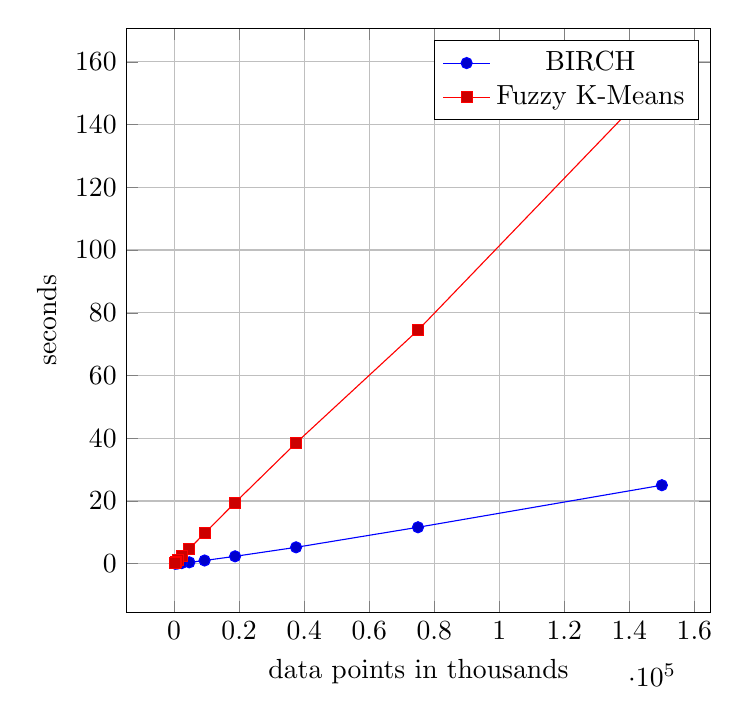
\begin{tikzpicture}
\begin{axis}[
    height=9cm,
    width=9cm,
    xlabel={data points in thousands},
    ylabel={seconds},
    grid=major,
  ]
  \addplot coordinates {
    (150000,25.030436)
    (75000,11.624714)
    (37500,5.232216)
    (18750,2.363530)
    (9375,1.031360)
    (4688,0.447284)
    (2344,0.203005)
    (1172,0.091562)
    (586,0.043213)
    (297,0.020289)
  };
  \addlegendentry{BIRCH}
  \addplot coordinates {
    (150000,155.195909)
    (75000,74.441829)
    (37500,38.501281)
    (18750,19.471102)
    (9375,9.723024)
    (4688,4.771375)
    (2344,2.414930)
    (1172,1.214021)
    (586,0.640441)
    (297,0.338978)
  };
  \addlegendentry{Fuzzy K-Means}
\end{axis}
\end{tikzpicture}
\end{center}



\begin{center}
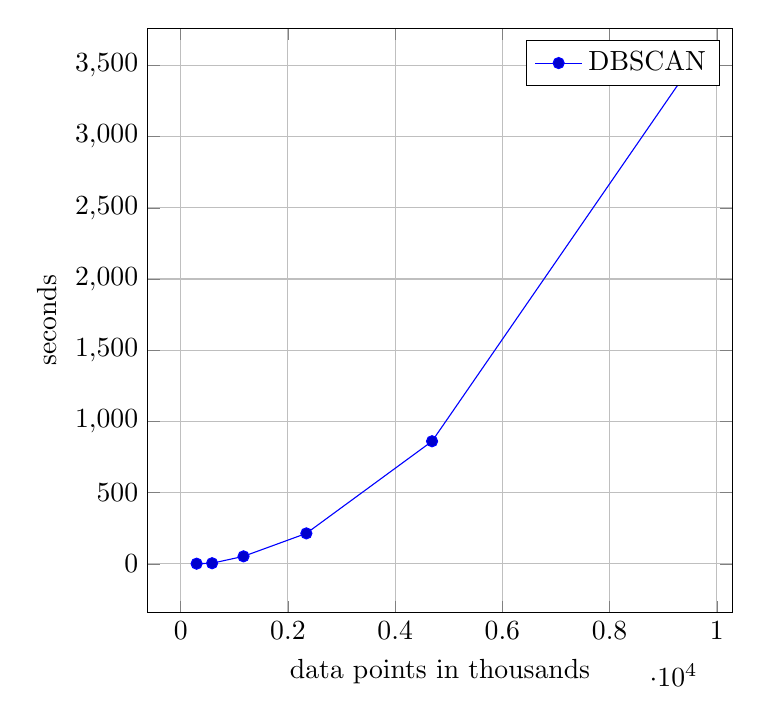
\begin{tikzpicture}
\begin{axis}[
    height=9cm,
    width=9cm,
    xlabel={data points in thousands},
    ylabel={seconds},
    grid=major,
  ]
  \addplot coordinates {
    (9375,3418.699)
    (4688,861.212)
    (2344,214.546)
    (1172,53.367)
    (586,5.066)
    (297,1.827)
  };
  \addlegendentry{DBSCAN}
\end{axis}
\end{tikzpicture}
\end{center}

% \begin{figure}[!hb]
%     \centering
%     \includegraphics[width=90mm]{dbscan_cluster.png}
%     \caption{DBSCAN result}
% \end{figure}

\section{Discussion and Conclusion}
The results of the empirical evaluation correlated well with the asymptotic time complexity with respect to each algorithm, with the exception of \texttt{DBSCAN}. The function calls related to the algorithm correlated well with the asymptotic time complexity without the R*-tree data structure, but the actual program running time was much larger and prohibited the completion of a subset of the dataset. In addition, the author was unable to use the R*-tree implementation in the DBSCAN implementation. Furthermore, \texttt{DBSCAN} is unable to handle clustering of data with a dimensionality greater than 2, and therefore suffering the curse of dimensionality. \cite{optimal}

\newpage
\begin{thebibliography}{1}

\bibitem{survey} R. Xu, D. Wunsch, ``Survey of Clustering Algorithms'', \emph{IEEE Transactions on Neural Networks}, vol. 16, no. 3, May, 2005, available at 
\url{http://axon.cs.byu.edu/Dan/678/papers/Cluster/Xu.pdf}.

\bibitem{spat} J. Burt, G. barber, D. Rugby.  ``Elementary Statistics for Geographers'', Guilford Publications, 2009.

\bibitem{spatial} E. Kolatch, ``Clustering Algorithms for Spatial Databases: A Survey'', \emph{unpublished}, available at
\url{http://mrl.cecsresearch.org/Resources/papers/Ericasurvey.pdf}

\bibitem{birch} T. Zhang, R. Ramakrishnan, M. Livny, ``BIRCH: An Efficient Data Clustering Method for Very Large Databases'', \emph{SIGMOD ’96}, available at
\url{http://citeseerx.ist.psu.edu/viewdoc/summary?doi=10.1.1.17.2504}

\bibitem{dbscan} M. Ester, H. Kriegel, J. Sander, X. Xu. ``A Density-Based Algorithm for Discovering Clusters in Large Spatial Databases with Noise'', \emph{2nd International Conference on Knowledge Discovery and Data Mining}

\bibitem{pattern} J. C. Bezdek ``Pattern Recognition with Fuzzy Objective Function Algorithm'', \emph{Press, New York}, 1981.

\bibitem{optimal} A. Hinneburg, D.A. Keim, ``Optimal Grid-Clustering: Towards Breaking the Curse of Dimensionality in High-Dimensional Clustering'', \emph{unpublished}, 1999, available at
\url{http://citeseerx.ist.psu.edu/viewdoc/download?doi=10.1.1.44.4721&rep=rep1&type=pdf} 

\bibitem{efficient} A. Denton, ``EFFICIENT HIERARCHICAL CLUSTERING OF LARGE DATA SETS USING P-TREES'', \emph{unpublished}, available at
\url{http://www.cs.ndsu.nodak.edu/~adenton/thesis/chapter7_Final.pdf}

\bibitem{fuzzy} Apache Foundation, ``Fuzzy K-means'', \emph{Apache Mahmout}, available at
\url{https://cwiki.apache.org/MAHOUT/fuzzy-K-Means.html}

\bibitem{literature} B.G.O. Reddy, M. Ussenaiah, ``Literature Survey On Clustering Techniques'', \emph{IOSR Journal of Computer Engineering}, vol. 3, iss. 1 (July-Aug. 2012), PP 01-12, available at
\url{http://iosrjournals.org/iosr-jce/full-issue/vol3-issue1.pdf}

\bibitem{data} C. Döring, M. J. Lesot, and R. Kruse, ``Data analysis with fuzzy clustering methods'', \emph{Computational Statistics and Data Analysis},2006, pp. 192-214.

\bibitem{hoffstein} Corey Hoffstein, ``DBSCAN'', \emph{Github.com}, available at
\url{https://github.com/choffstein/dbscan}

\bibitem{kmeans} C-T Chang, J.Z.C. Lai and M-D Jeng, ``A Fuzzy K-means clustering algorithm  using cluster center displacement'', \emph{Journal of information science and engineering} 27, 995-1009, 2011.

\bibitem{oberst} Jan Oberst, ``BIRCH'', \emph{Github.com}, available at
\url{https://github.com/janoberst/BIRCH/blob/master/birch.py}

\bibitem{suppressed} J. L. Fan, W. Z. Zhen, and W. X. Xie, ``Suppressed fuzzy c-means clustering algorithm'', \emph{ Recognition Letters}, 2003, pp. 1607-1612.

\bibitem{denisty} M. Parimala, D. Lopez, N.C. Senthilkumar, ``A Survey on Density Based Clustering Algorithms for Mining Large Spatial Databases'', \emph{International Journal of Advanced Science and Technology}, vol. 31, June, 2011, available at
\url{http://www.sersc.org/journals/IJAST/vol31/5.pdf}

\bibitem{comparative} M. Verma, M. Srivastava, N. Chack, A. K. Diswar, N. Gupta, ``A Comparative Study of Various Clustering Algorithms in Data Mining'', \emph{International Journal of Engineering Research and Applications}, vol. 2, iss. 3, May-Jun, 2012, pp.1379-1384, available at
\url{http://www.ijera.com/papers/Vol2_issue3/ID2313791384.pdf}

\bibitem{categorization} N. Soni, A. Ganatra, ``Categorization of Several Clustering Algorithms from Different Perspective: A Review'', \emph{International Journal of Advanced Research in Computer Science and Software Engineering}, vol. 2, iss. 8, August, 2012, available at
\url{http://www.ijarcsse.com/docs/papers/8_August2012/Volume_2_issue_8/V2I800161.pdf}

\bibitem{efficient} R. L. Cannon, J. V. Dave, and J. C. Bezdek, ``Efficient implementation of the fuzzy c- means clustering algorithm'', \emph{IEEE Transactions on PAMI}, Vol. 8, 1986, pp. 248-255.

\bibitem{extended} U. Kaymak, M. Setnes, ``Extended Fuzzy Clustering Algorithms'', \emph{Erasmus Research Institute of Management}, available at
\url{http://repub.eur.nl/res/pub/57/erimrs20001123094510.pdf}

\end{thebibliography}

% that's all folks
\end{document} 